\documentclass{article}
\usepackage[paperwidth=34.6cm,paperheight=22.4cm,margin=0cm]{geometry}
\usepackage{graphicx}
\usepackage{tikz}
\usepackage{pgfplots}
\pgfplotsset{compat=1.18}
\usepackage[T1]{fontenc}
\usepackage{lmodern}
\pagestyle{empty}
\definecolor{unetblue}{HTML}{163A75}
\definecolor{evidenceorange}{HTML}{D55E00}
\definecolor{fastteal}{HTML}{008577}
\definecolor{fcnnpurple}{HTML}{56236D}
\definecolor{heading}{HTML}{172B42}
\definecolor{muted}{HTML}{526173}
\pgfplotsset{
  unet/.style={unetblue,thick,dashed,mark=o,mark options={solid,fill=white},mark repeat=3,mark phase=1},
  evidence/.style={evidenceorange,thick,dotted,mark=square,mark options={solid,fill=white},mark repeat=3,mark phase=2},
  fast/.style={fastteal,thick,mark=triangle,mark options={solid,fill=white},mark repeat=3,mark phase=3},
  fcnn/.style={fcnnpurple,thick,dashdotted,mark=diamond,mark options={solid,fill=white},mark repeat=3},
}
\newcommand{\plotours}{%
 \addplot[unet] table[x=snr,y=unet]{data/scores.dat};
 \addplot[evidence] table[x=snr,y=evidence]{data/scores.dat};
 \addplot[fast] table[x=snr,y=fast]{data/scores.dat};
}
\begin{document}
\noindent
\begin{tikzpicture}[x=1cm,y=1cm,font=\sffamily]
\path[use as bounding box] (0,0) rectangle (34.5,22.2);
\node[anchor=west,text=heading,font=\sffamily\bfseries\fontsize{23}{27}\selectfont]
 at (1.3,21.25) {Our models on the paper's Figure 16a};
\node[anchor=west,text=muted,font=\sffamily\large] at (1.3,20.1)
 {Original published graph retained --- our results added as thick lines with markers};

% Unmodified crop of the original published figure.
% Crop in PDF points: (64,56)-(273,221), page 12.
% Thus width=21cm and height=21*165/209 cm.
\node[anchor=south west,inner sep=0] at (0.8,3.7)
 {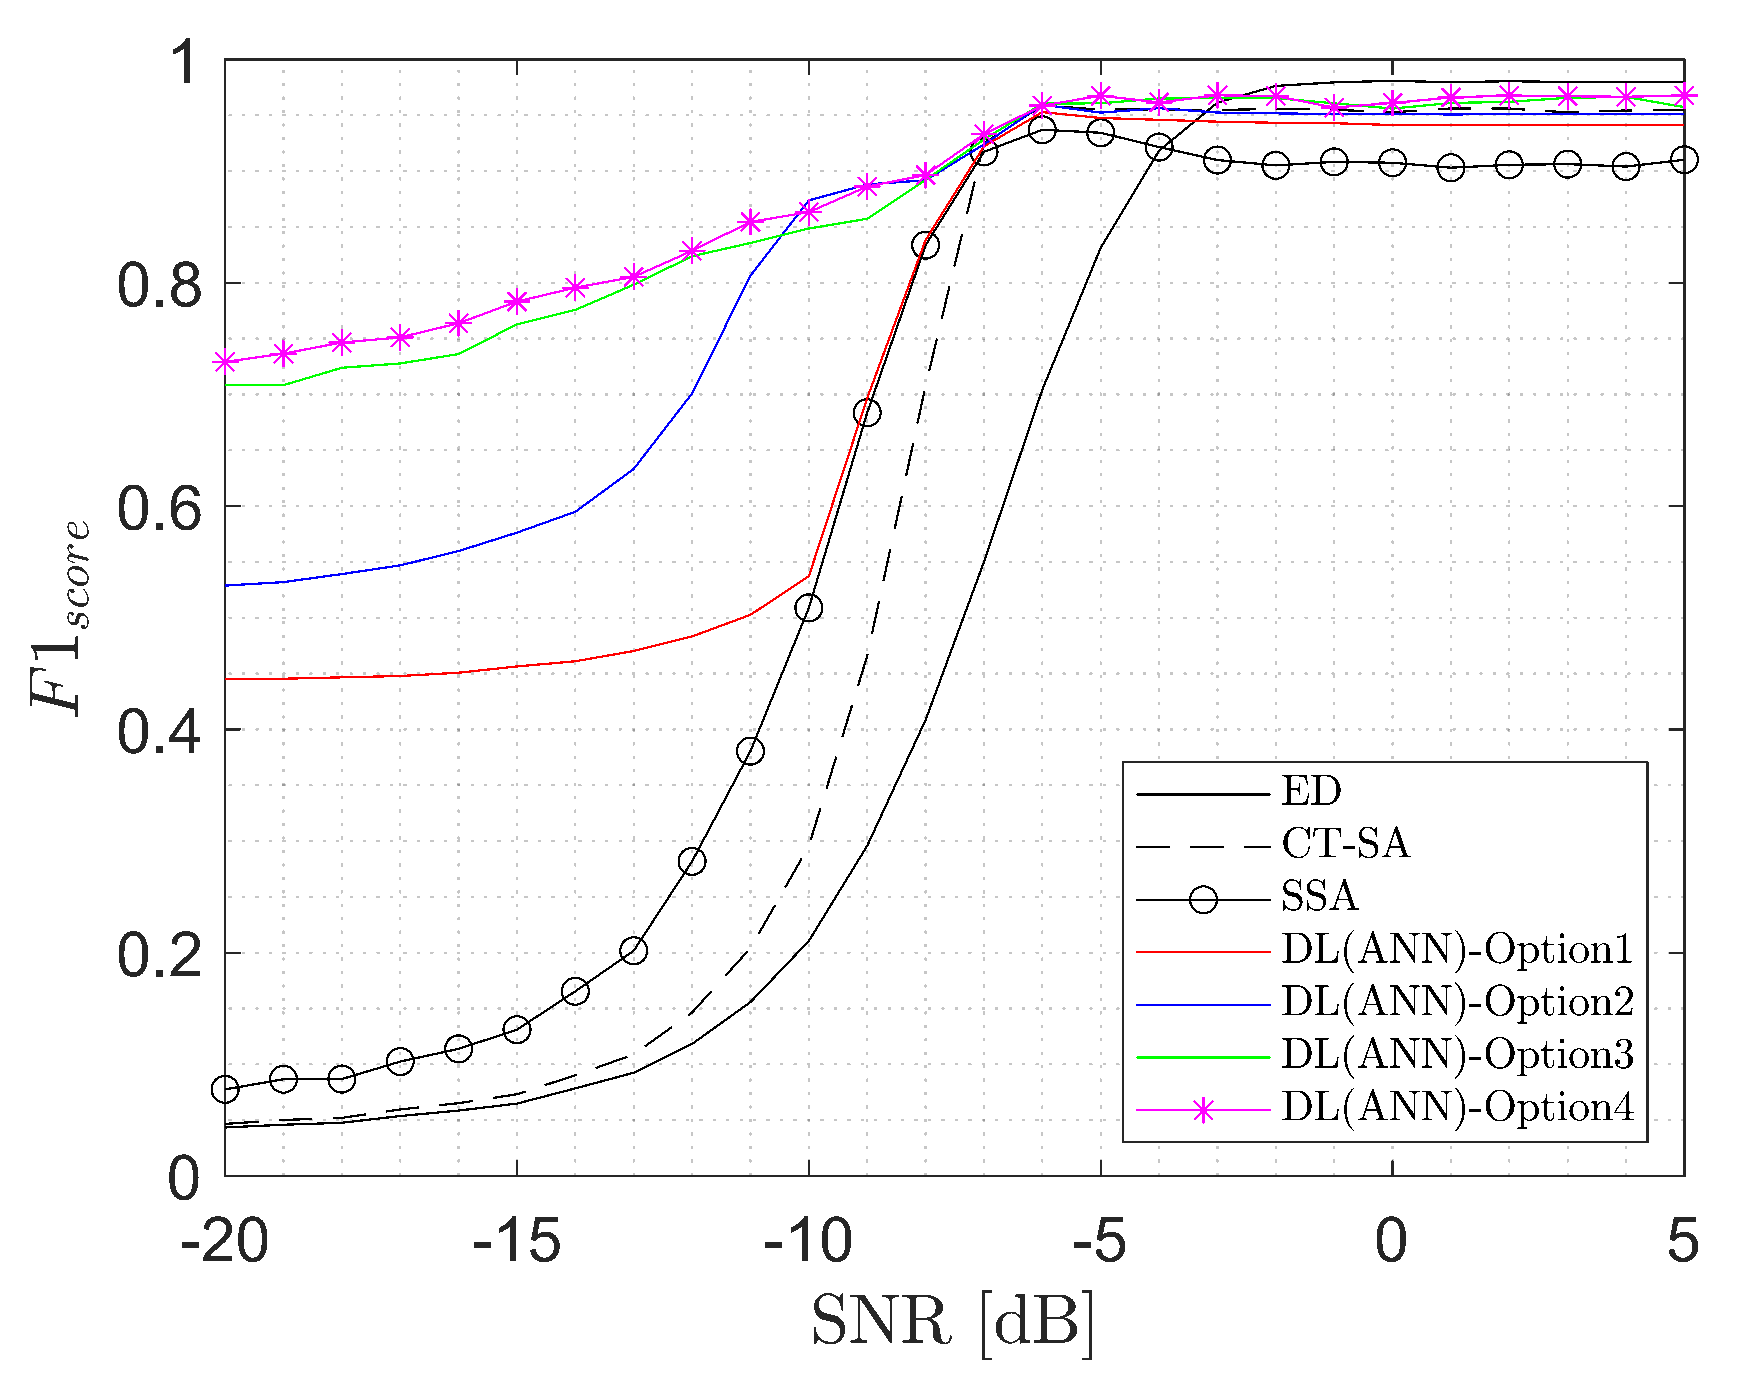
\includegraphics[width=21cm]{images/figure16a_original.png}};

% Align exactly with source axes, rather than estimating placement by eye.
% Axis bounds in source PDF points:
% left=90.9735, right=266.0925, top=63.0485, bottom=197.0105.
\begin{axis}[
 at={(3.510256cm,6.110428cm)},anchor=south west,
 width=17.595689cm,height=13.460297cm,scale only axis,
 xmin=-20,xmax=5,ymin=0,ymax=1,
 hide axis,clip=false,mark size=2.6pt,
 legend style={draw=none,font=\sffamily\large,fill=white,
   at={(1.16,0.98)},anchor=north west,cells={anchor=west},row sep=8pt},
]
\plotours
\addplot[fcnn] table[x=snr,y=fcnn]{data/scores.dat};
\legend{Original U-Net,EvidenceAxialNet,FastUNet,FCNN recreation*}
\end{axis}

\node[anchor=west,text=heading,font=\sffamily\bfseries\large] at (24,18.8) {OUR RESULTS};
\node[anchor=north west,text=muted,align=left] at (24,13.8)
 {The legend inside the original graph\\identifies the paper's thin curves.};

\begin{axis}[
 at={(24.6cm,6.0cm)},anchor=south west,
 width=8.2cm,height=6.1cm,scale only axis,
 title={Low-SNR detail: our three models},
 title style={font=\sffamily\small},
 xmin=-20.3,xmax=-11.7,ymin=0.765,ymax=0.95,
 xlabel={SNR (dB)},ylabel={F1 score},
 xtick={-20,-18,-16,-14,-12},ytick={0.78,0.82,0.86,0.90,0.94},
 grid=major,grid style={gray!15},axis lines=left,
 tick label style={font=\sffamily\small},
 mark size=2pt,
]
\plotours
\end{axis}
\node[anchor=north west,text=muted,align=left] at (24,4.1)
 {Near-overlapping lines mean similar scores.\\No values have been shifted or smoothed.};
\node[anchor=west,font=\sffamily\small] at (1.3,2.15)
 {Source: Alammar \& L\'opez-Ben\'itez (2023), Figure 16a, AWGN. DOI: 10.1016/j.phycom.2023.102113};
\node[anchor=west,font=\sffamily\small] at (1.3,1.4)
 {Local results: mean per-image pixel F1. Training data and evaluation protocols differ from the paper.};
\node[anchor=west,font=\sffamily\small] at (1.3,0.65)
 {* FCNN recreation is our earlier experiment on a separate test set; it is not the published paper curve.};
\end{tikzpicture}
\end{document}
